\uuid{e0p4}
\exo7id{5910}
\auteur{rouget}
\organisation{exo7}
\datecreate{2010-10-16}
\isIndication{false}
\isCorrection{true}
\chapitre{Intégration}
\sousChapitre{Intégrale multiple}

\contenu{
\texte{
Soient $(p_1,p_2,q_1,q_2)\in]0,+\infty[^4$ tel que $p_1<p_2$ et $q_1<q_2$.

Calculer l'aire du domaine $D=\{(x,y)\in\Rr^2/\;2p_1x\leqslant y^2\leqslant2p_2x\;\text{et}\;2q_2y\leqslant x^2\leqslant2q_2y\}$.
}
\reponse{
\ 
$$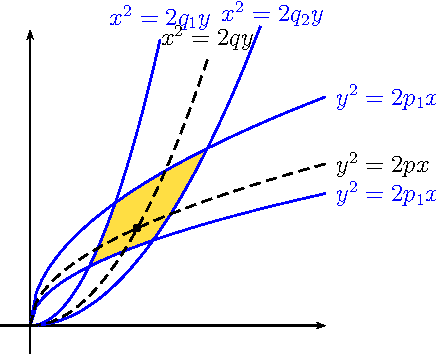
\includegraphics{../images/img005910-1}$$


L'aire du domaine considéré $D=\{(x,y)\in\Rr^2/\;2p_1x\leqslant y^2\leqslant 2p_2x\;\text{et}\;2q_2y\leqslant x^2\leqslant2q_2x\}$ est

\begin{center}
$\mathcal{A}=\displaystyle\iint_{D}dxdy$.
\end{center}

Pour $(x,y)\in D^2$, posons $p= \frac{y^2}{2x}$ et $q= \frac{x^2}{2y}$ ou encore considérons l'application $\begin{array}[t]{cccc}
\varphi~:&D&\rightarrow&[p_1,p_2]\times[q_1,q_2]\\
 &(x,y)&\mapsto&\left( \frac{y^2}{2x}, \frac{x^2}{2y}\right)
 \end{array}$ et vérifions que $\varphi$ est un $C^1$-difféomorphisme.
 
 

 

\textbullet~Pour chaque $(x,y)\in D^2$, on $2p_1x\leqslant y^2\leqslant 2p_2x$ et $2q_1y\leqslant x^2\leqslant2q_2y$ ou encore $p_1\leqslant \frac{y^2}{2x}\leqslant p_2$ et $q_1\leqslant \frac{x^2}{2y}\leqslant q_2$. Donc $\varphi$ est bien une application.

\textbullet~Soit $(p,q)\in[p_1,p_2]\times[q_1,q_2]$. Pour $(x,y)\in(]0,+\infty[)^2$,

\begin{center}
$\left\{
\begin{array}{l}
 \frac{y^2}{2x}=p\\
\rule{0mm}{7mm} \frac{x^2}{2y}=q
\end{array}
\right.\Leftrightarrow\left\{
\begin{array}{l}
y= \frac{x^2}{2q}\\
\rule{0mm}{7mm} \frac{(x^2/2q)^2}{2x}=p
\end{array}
\right.\Leftrightarrow\left\{
\begin{array}{l}
x=\sqrt[3]{8pq^2}\\
y=\sqrt[3]{8p^2q}
\end{array}
\right.$
\end{center}

Donc, l'équation $\varphi(x,y)=(p,q)$ a exactement une solution $(x_0,y_0)$ dans $]0,+\infty[^2$. De plus, puisque $ \frac{y_0^2}{2x_0}=p\in[p_1,p_2]$ et $ \frac{x_0^2}{2y_0}=q\in[q_1,q_2]$, on a $2p_1x_0\leqslant y_0^2\leqslant 2p_2x_0$ et $2q_1y_0\leqslant x_0^2\leqslant 2q_2y_0$ et donc $(x_0,y_0)\in D^2$. Donc $\varphi$ est une bijection.

\textbullet~$\varphi$ est de classe $C^1$ sur $D$ et pour $(x,y)\in D^2$,

\begin{center}
$ \frac{D(p,q)}{D(x,y)}=J(\varphi)(x,y)=\left|
\begin{array}{cc}
- \frac{y^2}{2x^2}& \frac{y}{x}\\
 \frac{x}{y}&- \frac{x^2}{2y^2}
\end{array}
\right|= \frac{1}{4}-1=- \frac{3}{4}\neq0$.
\end{center}

Ainsi, $\varphi$ est une bijection de $D$ sur $[p_1,p_2]\times[q_1,q_2]$, de classe $C^1$ sur $D$ et son jacobien ne s'annule pas sur $D$. On sait alors que $\varphi$ est un $C^1$-difféomorphisme de $D$ sur $[p_1,p_2]\times[q_1,q_2]$.

Posons alors $(p,q)=\varphi(x,y)$ dans $\displaystyle\iint_{D}dxdy$. On obtient

\begin{center}
$\mathcal{A}=\displaystyle\iint_{D}dxdy=\displaystyle\iint_{[p_1,p_2]\times[q_1,q_2]}\left| \frac{D(x,y)}{D(p,q)}\right|dpdq=\displaystyle \frac{4}{3}\iint_{[p_1,p_2]\times[q_1,q_2]}dpdq= \frac{4}{3}(p_2-p_1)(q_2-q_1)$.
\end{center}

\begin{center}
\shadowbox{
$\mathcal{A}= \frac{4}{3}(p_2-p_1)(q_2-q_1)$.
}
\end{center}
}
}
